\documentclass[../notes.tex]{subfiles}

\pagestyle{main}
\renewcommand{\chaptermark}[1]{\markboth{\chaptername\ \thechapter\ (#1)}{}}
\setcounter{chapter}{11}

\begin{document}




\chapter{Experimental Kinetics}
\section{Kinetics of Catalytic Reactions}
\begin{itemize}
    \item \marginnote{11/19:}Last week's lectures.
    \begin{itemize}
        \item Very simple kinetic scenarios.
        \item Linearizations allows us to extract essential kinetic parameters for reactions.
        \item Kinetic descriptions for multistep processes.
        \item Steady-state approximation, quasi-equilibrium approximation.
    \end{itemize}
    \item Today: Kinetics of Catalytic Reactions.
    \item Catalysts speed up the rate of reaction without altering the thermodynamics.
    \item Consider the following balanced chemical reaction.
    \begin{equation*}
        \ce{A + B + cat -> P + cat}
        \qquad\equiv\qquad
        \ce{A + B ->[cat] P}
    \end{equation*}
    \begin{itemize}
        \item Since the catalyst appears on both sides of the reaction, we typically write it over the arrow.
        \item This notational simplification alides a great deal of multistep complexity.
    \end{itemize}
    \item Consider a hypothetical potential energy surface.
    \begin{figure}[h!]
        \centering
        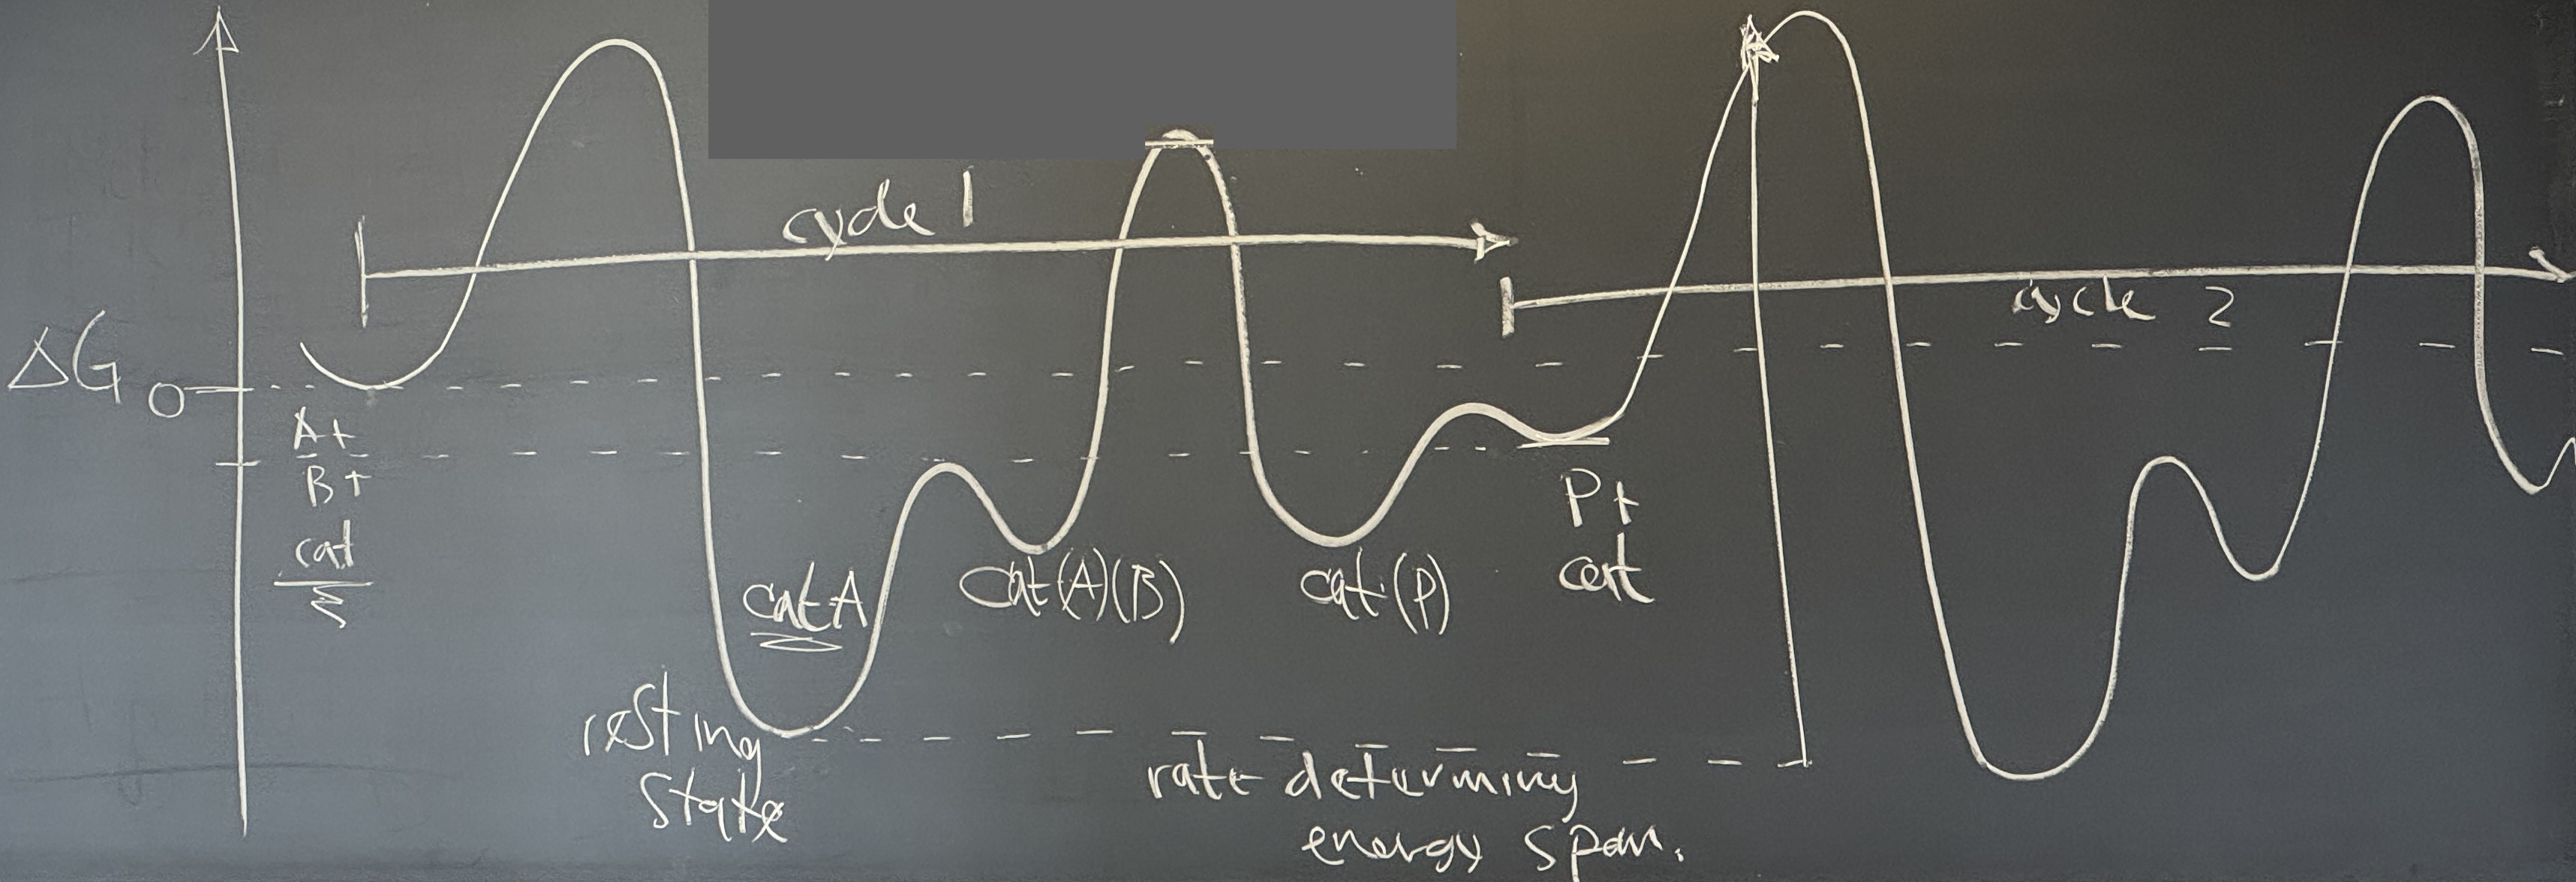
\includegraphics[width=0.8\linewidth]{modelCatPES.JPG}
        \caption{Model catalytic potential energy surface.}
        \label{fig:modelCatPES}
    \end{figure}
    \begin{itemize}
        \item Define a reference energy as zero; suppose the starting materials (\ce{A + B + cat}) begin here.
        \item Suppose, then, that they proceed through a multistep potential energy surface along our reaction coordinate.
        \item If this were a stoichiometric reaction, the first step would be rate-determining (highest energy barrier), and the first intermediate would be the product (lowest energy species).
        \begin{itemize}
            \item But we're catalytic, so we have to consider cycles 2, 3, \dots
            \item These cycles are driven forward by the ever-so-slight difference in energy $\Delta G$ between starting materials and products.
        \end{itemize}
        \item The "first intermediate" is actually the catalyst \textbf{resting state}.
        \begin{itemize}
            \item Indeed, the thing that we throw in may not be the dominant species in solution!
            \item It could be \ce{cat*(A)}, \ce{cat*(A)(B)}, or \ce{cat*(P)}!
        \end{itemize}
        \item Similarly, the difference in energy between the lowest valley and highest peak is the \textbf{rate-determining energy span}.
        \item Reference (good description of rate-determining energy span): \textcite{bib:modelCatPES}.
    \end{itemize}
    \item Because continuous potential energy surfaces are not great representations, we typically view catalysts as acting in \textbf{catalytic cycles}.
    \begin{figure}[h!]
        \centering
        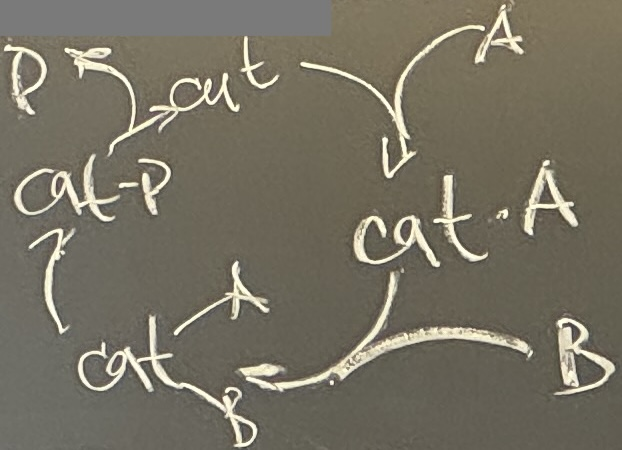
\includegraphics[width=0.23\linewidth]{modelCatCycle.JPG}
        \caption{Model catalytic cycle.}
        \label{fig:modelCatCycle}
    \end{figure}
    \begin{itemize}
        \item This is not that uncommon a catalytic cycle to find!
    \end{itemize}
    \item Let's now do a kinetic analysis of this model catalytic cycle, using some of the tools developed last lecture.
    \begin{figure}[h!]
        \centering
        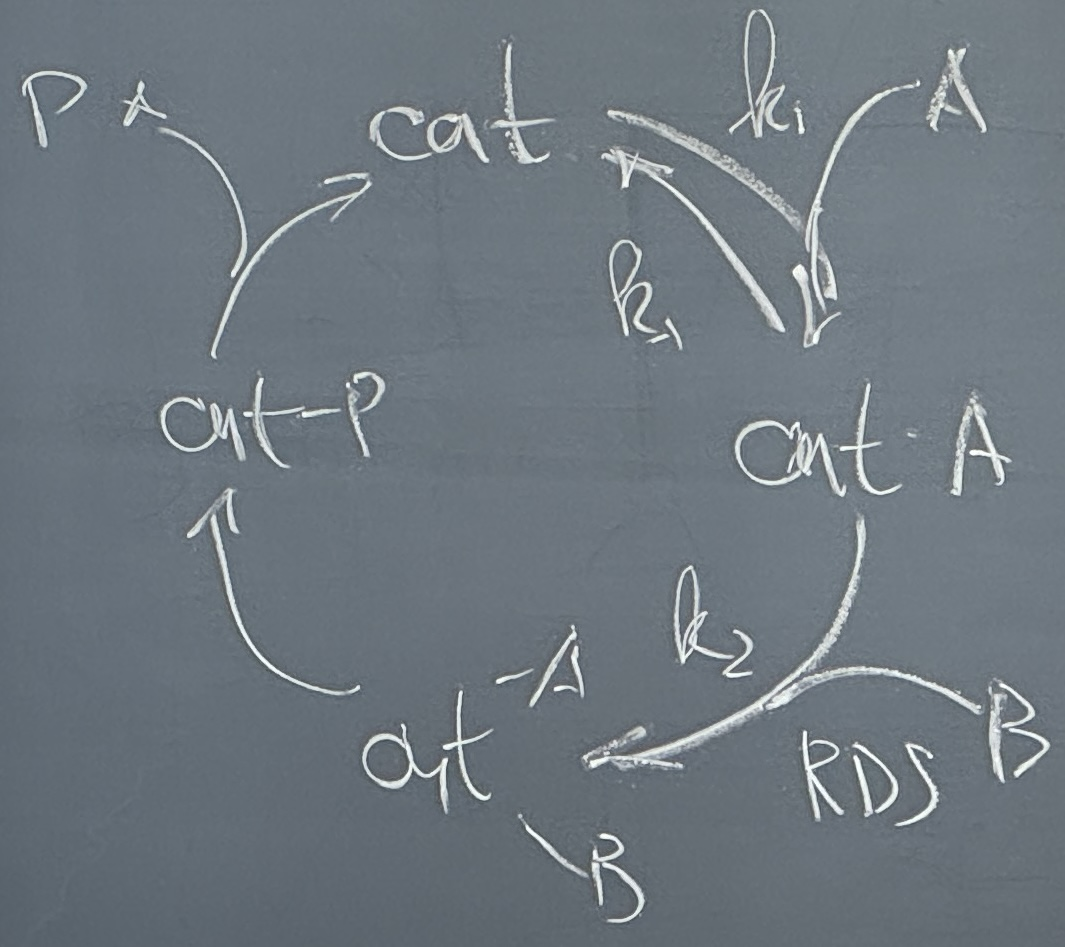
\includegraphics[width=0.3\linewidth]{modelCatCycleKin.JPG}
        \caption{Model catalytic cycle (kinetic analysis).}
        \label{fig:modelCatCycleKin}
    \end{figure}
    \begin{itemize}
        \item Assume that the first step is a reversible binding to \ce{A}.
        \item Recall that the rate-determining step follows the resting state. Thus,
        \begin{equation*}
            \rate = \dv{\cnc{P}}{t}
            = -\dv{\cnc{A}}{t}
            = k_2\cnc{cat*A}\cnc{B}
        \end{equation*}
        \item We can then apply our rule of thumb for the steady-state approximation.
        \begin{equation*}
            \rate = \frac{k_1k_2\cnc{A}\cnc{B}\cnc{cat}}{k_{-1}+k_2\cnc{B}}
        \end{equation*}
    \end{itemize}
    \item Going forward, it will be useful to define the total concentration of catalyst
    \begin{equation*}
        \cnc[T]{cat} := \cnc{cat}+\cnc{cat*A}+\cnc{cat*AB}+\cnc{cat*P}
    \end{equation*}
    \begin{itemize}
        \item To derive the rate law for Figure \ref{fig:modelCatCycleKin} in terms of $\cnc[T]{cat}$ --- an observable --- we'd need a system of equations.
    \end{itemize}
    \item Let's now consider a different (simpler) catalytic cycle to develop some core ideas.
    \begin{figure}[h!]
        \centering
        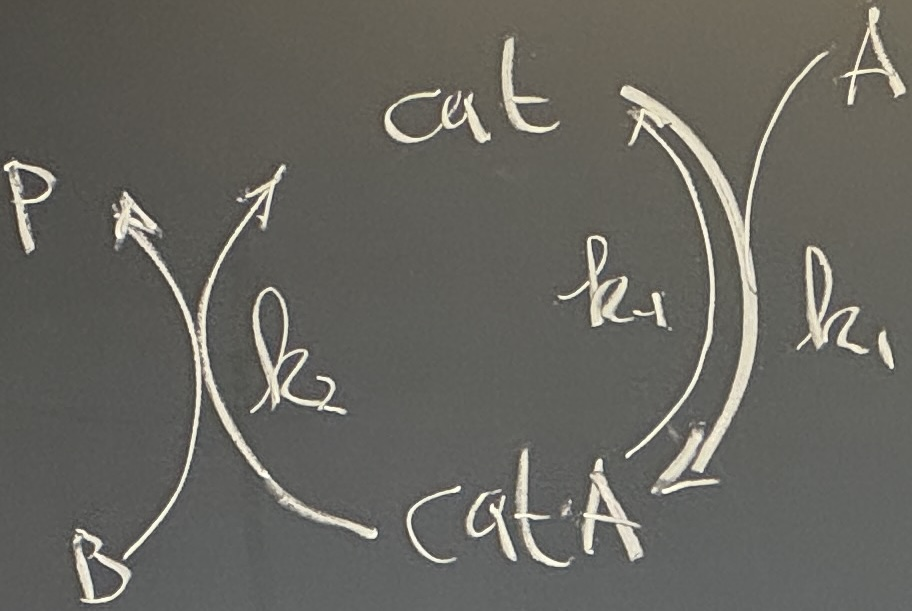
\includegraphics[width=0.23\linewidth]{modelCat2Kin.JPG}
        \caption{Model two-step catalytic cycle (kinetic analysis).}
        \label{fig:modelCat2Kin}
    \end{figure}
    \begin{itemize}
        \item This cycle pertains to a reaction
        \begin{equation*}
            \ce{A + B ->[cat] P}
        \end{equation*}
        \item If the second step is rate-determining, then
        \begin{equation*}
            \rate = k_2\cnc{cat*A}\cnc{B}
        \end{equation*}
        \item It will also be useful to have the assumption
        \begin{equation*}
            \cnc[T]{cat} = \cnc{cat}+\cnc{cat*A}
        \end{equation*}
    \end{itemize}
    \item Let's now evaluate this catalytic cycle using the quasi-equilibrium assumption.
    \begin{itemize}
        \item Warning: Lots of algebra coming up!
        \begin{itemize}
            \item Squiggly lines on the board mean abbreviations.
        \end{itemize}
        \item The quasi-equilibrium assumption tells us that
        \begin{equation*}
            K = \frac{k_1}{k_{-1}}
            = \frac{\cnc{cat*A}}{\cnc{cat}\cnc{A}}
        \end{equation*}
        \item We first solve for the concentration of the catalyst.
        \begin{equation*}
            \cnc{cat} = \frac{\cnc{cat*A}}{K\cnc{A}}
        \end{equation*}
        \item We can drop this into our expression for the total catalyst.
        \begin{equation*}
            \cnc[T]{cat} = \frac{\cnc{cat*A}}{K\cnc{A}}+\cnc{cat*A}
        \end{equation*}
        \item We can factor out the $\cnc{cat*A}$'s.
        \begin{equation*}
            \cnc[T]{cat} = \cnc{cat*A}\left( \frac{1}{K\cnc{A}}+1 \right)
        \end{equation*}
        \item Rearrange this to solve for $\cnc{cat*A}$.
        \begin{equation*}
            \cnc{cat*A} = \frac{\cnc[T]{cat}}{1/K\cnc{A}+1}
        \end{equation*}
        \item Remove this fractional denominator via multiplication by a clever form of 1 (namely, $K\cnc{A}/K\cnc{A}$).
        \begin{equation*}
            \cnc{cat*A} = \frac{K\cnc{A}\cnc[T]{cat}}{1+K\cnc{A}}
        \end{equation*}
        \item We can now drop this back into the rate expression to get an expression for the rate in terms of the overall catalyst concentration, which is more useful because that's an observable (we know how much we put in!).
        \begin{equation*}
            \rate = \frac{k_2K\cnc{A}\cnc{B}\cnc[T]{cat}}{1+K\cnc{A}}
        \end{equation*}
        \item Note that we could also write the $K$'s above as $\Keq$'s.
    \end{itemize}
    \item Let's now derive an analogous expression for the catalytic cycle in Figure \ref{fig:modelCat2Kin}, but this time under the steady-state approximation.
    \begin{itemize}
        \item We initially obtain
        \begin{equation*}
            \cnc{cat*A} = \frac{k_1\cnc{A}\cnc{cat}}{k_{-1}+k_2\cnc{B}}
        \end{equation*}
        \item Rearranging yields
        \begin{equation*}
            \cnc{cat} = \frac{\cnc{cat*A}(k_{-1}+k_2\cnc{B})}{k_1\cnc{A}}
        \end{equation*}
        \item Using the fact that $\cnc{cat}=\cnc[T]{cat}-\cnc{cat*A}$, we obtain
        \begin{equation*}
            \frac{\cnc{cat*A}(k_{-1}+k_2\cnc{B})}{k_1\cnc{A}} = \cnc[T]{cat}-\cnc{cat*A}
        \end{equation*}
        \item We get rid of the denominator by multiplying both sides by $k_1\cnc{A}$, collect a couple of terms, and rearrange into
        \begin{equation*}
            \cnc{cat*A}(k_1\cnc{A}+k_{-1}+k_2\cnc{B}) = k_1\cnc{A}\cnc[T]{cat}
        \end{equation*}
        \item Then divide both sides by the term in parentheses on the left.
        \begin{equation*}
            \cnc{cat*A} = \frac{k_1\cnc{A}\cnc[T]{cat}}{k_1\cnc{A}+k_{-1}+k_2\cnc{B}}
        \end{equation*}
        \item This substitution can now be dropped back into our rate law.
        \begin{align*}
            \rate &= k_2\cnc{cat*A}\cnc{B}\\
            &= \frac{k_1k_2\cnc{A}\cnc{B}\cnc[T]{cat}}{k_{-1}+k_2\cnc{B}+k_1\cnc{A}}
        \end{align*}
        \item We now multiply by another clever form of 1 (namely the inverse of $k_{-1}$ on both top and bottom).
        \begin{equation*}
            \rate = \frac{\frac{k_1}{k_{-1}}k_2\cnc{A}\cnc{B}\cnc[T]{cat}}{1+\frac{k_2}{k_{-1}}\cnc{B}+\frac{k_1}{k_{-1}}\cnc{A}}
        \end{equation*}
        \begin{itemize}
            \item This is known as the \textbf{one plus rate form} of the rate law because of the "$1+$" in the denominator.
        \end{itemize}
    \end{itemize}
    \item We can now compare the two rate laws we've derived.
    \begin{itemize}
        \item We do this by assuming that $k_{-1}\gg k_2$, which is exactly the scenario in which the quasi-equilibrium assumption would apply!
        \item We approach a limit where we can ignore the $k_2/k_{-1}$ term in the denominator, and $k_1/k_{-1}=\Keq$ (as established previously).
    \end{itemize}
    \item Let's consider some limiting scenarios.
    \begin{itemize}
        \item This will help us partially eliminate complexity.
        \item First, let's consider the scenario in which
        \begin{equation*}
            1 \gg \frac{k_2}{k_{-1}}\cnc{B} \approx \frac{k_1}{k_{-1}}\cnc{A}
        \end{equation*}
        \begin{itemize}
            \item In this case, the denominator vanishes and the simplified rate law is
            \begin{equation*}
                \rate = \frac{k_1}{k_{-1}}\cnc{A}\cnc{B}\cnc[T]{cat}
            \end{equation*}
            \item Since this constraint implies that $k_{-1}\gg k_2$, the second step must be rate-determining.
            \item It also follows that $\cnc[T]{cat}\approx\cnc{cat}$, and hence the resting state of the catalyst is the unbound catalyst!
            \item We can also say that the second step is \textbf{turnover-limiting}.
        \end{itemize}
        \item Second, let's consider the scenario in which
        \begin{equation*}
            \frac{k_2}{k_{-1}}\cnc{B} \gg \text{others}
        \end{equation*}
        \begin{itemize}
            \item By "others," we mean the other two terms in the denominator.
            \item In this case, the simplified rate law is
            \begin{equation*}
                \rate = k_1\cnc{A}\cnc[T]{cat}
            \end{equation*}
            \item This constraint implies that the first step is rate-determining.
            \item Hence, the reaction with \ce{B} (zero-order) is post-rate limiting.
            \item It follows additionally that once again, the resting state of the catalyst is the unbound catalyst!
        \end{itemize}
        \item Third, let's consider the scenario in which
        \begin{equation*}
            \frac{k_1}{k_{-1}}\cnc{A} \gg \text{others}
        \end{equation*}
        \begin{itemize}
            \item In this case, the simplified rate law is
            \begin{equation*}
                \rate = k_2\cnc{B}\cnc[T]{cat}
            \end{equation*}
            \item Zero-order dependence on $\cnc{A}$ implies that the catalyst is fully saturated with $\cnc{A}$.
            \item Hence, the second step is rate-determining and the resting state is the bound catalyst.
        \end{itemize}
        \item Fourth, everything matters.
        \begin{itemize}
            \item This scenario is not limiting but is, unfortunately, common.
            \item This implies a kinetic pathway in which all species are at roughly similar energies with roughly similar transition structures.
            \item This is often a good thing for catalysis, but we'll get there.
        \end{itemize}
    \end{itemize}
    \item Aside: The one plus rate form.
    \begin{equation*}
        \rate = \frac{c_1\cnc{A}\cnc{B}\cnc[T]{cat}}{1+c_2\cnc{A}+c_3\cnc{A}\cnc{B}+c_4\cnc{P}}
    \end{equation*}
    \begin{itemize}
        \item The rate law takes on the above general structure.
        \item We have a constant (the "kinetic term") $c$ modified by the concentrations of the inputs in the numerator, collectively referred to as the potential terms (because they reflect something about the TST with respect to the ground state).
        \item The denominator --- the \textbf{adsorption term} --- consists of all the forms that the catalyst can take.
        \item What do the constants tell us?
        \begin{itemize}
            \item $c_1$ tells us about the naked catalyst.
            \item $c_2\cnc{A}$ can tell us about the \ce{cat*A} complex.
            \item $c_3\cnc{A}\cnc{B}$ can tell us about the \ce{cat*AB} complex.
            \item $c_4\cnc{P}$ can tell us about the \ce{cat*P} complex.
        \end{itemize}
        \item Goal of this exercise: Gain intution for the algebra.
        \begin{itemize}
            \item The best kineticists can easily see the chemistry in rate laws the way that most organic chemists can see it in Lewis structures.
            \begin{itemize}
                \item Donna Blackmond at Scripps is one of Alex's favorite kineticists.
            \end{itemize}
            \item Similarly, spectroscopists can see chemistry in derivative waveforms; "what a power to have!"
        \end{itemize}
    \end{itemize}
    \item How do we increase the rate, i.e., max out the rate law?
    \begin{itemize}
        \item We want to get the denominator to go away.
        \item This gives Scenario 3, in which all of the substrate is bound to the catalyst and it's doing it's thing as fast as it can.\footnote{Why should this scenario give the fastest rate??}
        \begin{equation*}
            \rate_\text{max} = k_2\cnc{B}\cnc[T]{cat}
        \end{equation*}
    \end{itemize}
    \item Let's plop $\rate_\text{max}$ into our steady-state approximation rate law, and multiply it by $1=k_{-1}/k_{-1}$.
    \begin{equation*}
        \rate = \frac{\rate_\text{max}k_1\cnc{A}}{k_{-1}+k_2\cnc{B}+k_1\cnc{A}}
    \end{equation*}
    \begin{itemize}
        \item Now define
        \begin{equation*}
            \frac{1}{K_m} = \frac{k_1}{k_{-1}+k_2\cnc{B}}
        \end{equation*}
        \item It follows that
        \begin{equation*}
            \rate = \frac{\rate_\text{max}\cnc{A}}{K_m+\cnc{A}}
        \end{equation*}
    \end{itemize}
    \item Under the quasi-equilibrium assumption, we can assume something else.
    \begin{equation*}
        \rate = \frac{\rate_\text{max}\Keq\cnc{A}}{1+\Keq\cnc{A}}
    \end{equation*}
    \begin{itemize}
        \item Now define
        \begin{equation*}
            K_D = \frac{1}{\Keq}
        \end{equation*}
        as the dissociation constant for the \ce{cat*A} complex.
        \item It follows that
        \begin{equation*}
            \rate = \frac{\rate_\text{max}\cnc{A}}{K_D+\cnc{A}}
        \end{equation*}
    \end{itemize}
    \item $K_m$ takes us into \textbf{Michaelis-Menten kinetics}.
    \begin{itemize}
        \item Defined in the early twentieth century to guide our emerging understanding of biochemical kinetics.
        \item Using the historical nomenclature (substrate and enzyme), we have
        \begin{equation*}
            \ce{S + E <=>[$k_f$][$k_r$] S*E ->[$k_\text{cat}$] P}
        \end{equation*}
        \item There is a relationship here to saturation kinetics, defined in the limiting scenarios with Figure \ref{fig:modelCat2Kin}.
        \item Michaelis and Menten talked about a kinetic velocity $v_\text{max}$ where we go from asymptotic speed down to a first-order dependence on $\cnc{S}$.
        \item Other relevant expressions:
        \begin{align*}
            K_m &= \frac{k_r+k_\text{cat}}{k_f}&
            v &= \frac{v_\text{max}\cnc{S}}{K_m+\cnc{S}}
        \end{align*}
        \item If $K_m=\cnc{S}$, then $v=v_\text{max}/2$.
        \item We can experimentally determine the Michaelis constant by assaying a bunch of different initial rates at different concentrations.
    \end{itemize}
    \item What's the point of Michaelis-Menten kinetics?
    \begin{figure}[h!]
        \centering
        \begin{subfigure}[b]{0.4\linewidth}
            \centering
            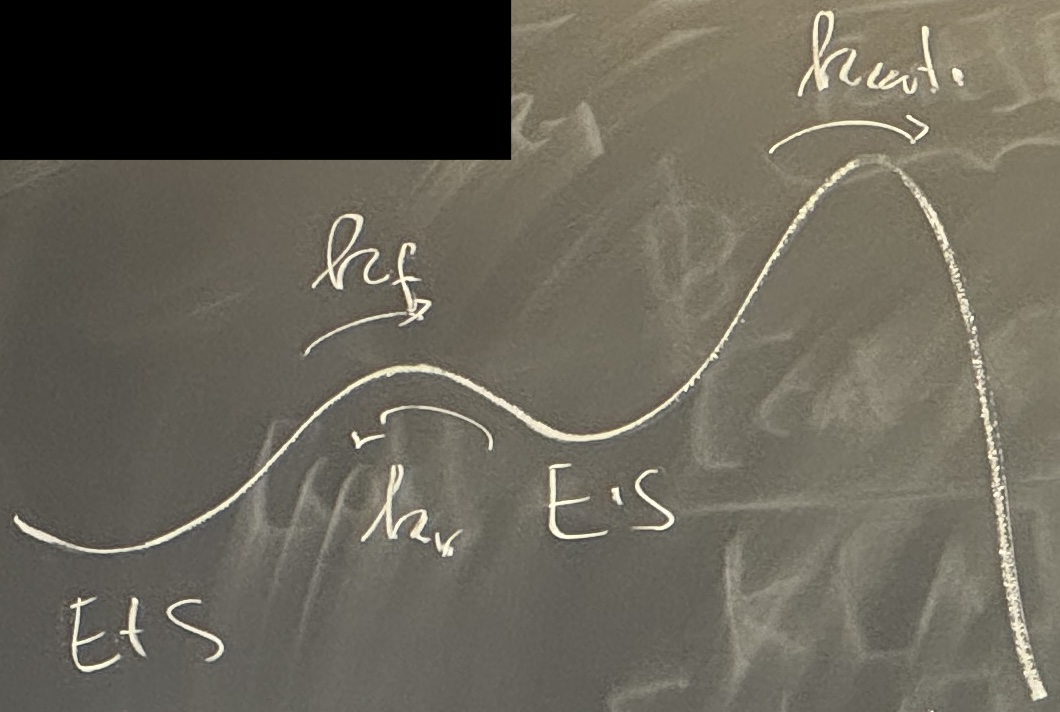
\includegraphics[width=0.8\linewidth]{MMkina.JPG}
            \caption{Zeroeth-order.}
            \label{fig:MMkina}
        \end{subfigure}
        \begin{subfigure}[b]{0.4\linewidth}
            \centering
            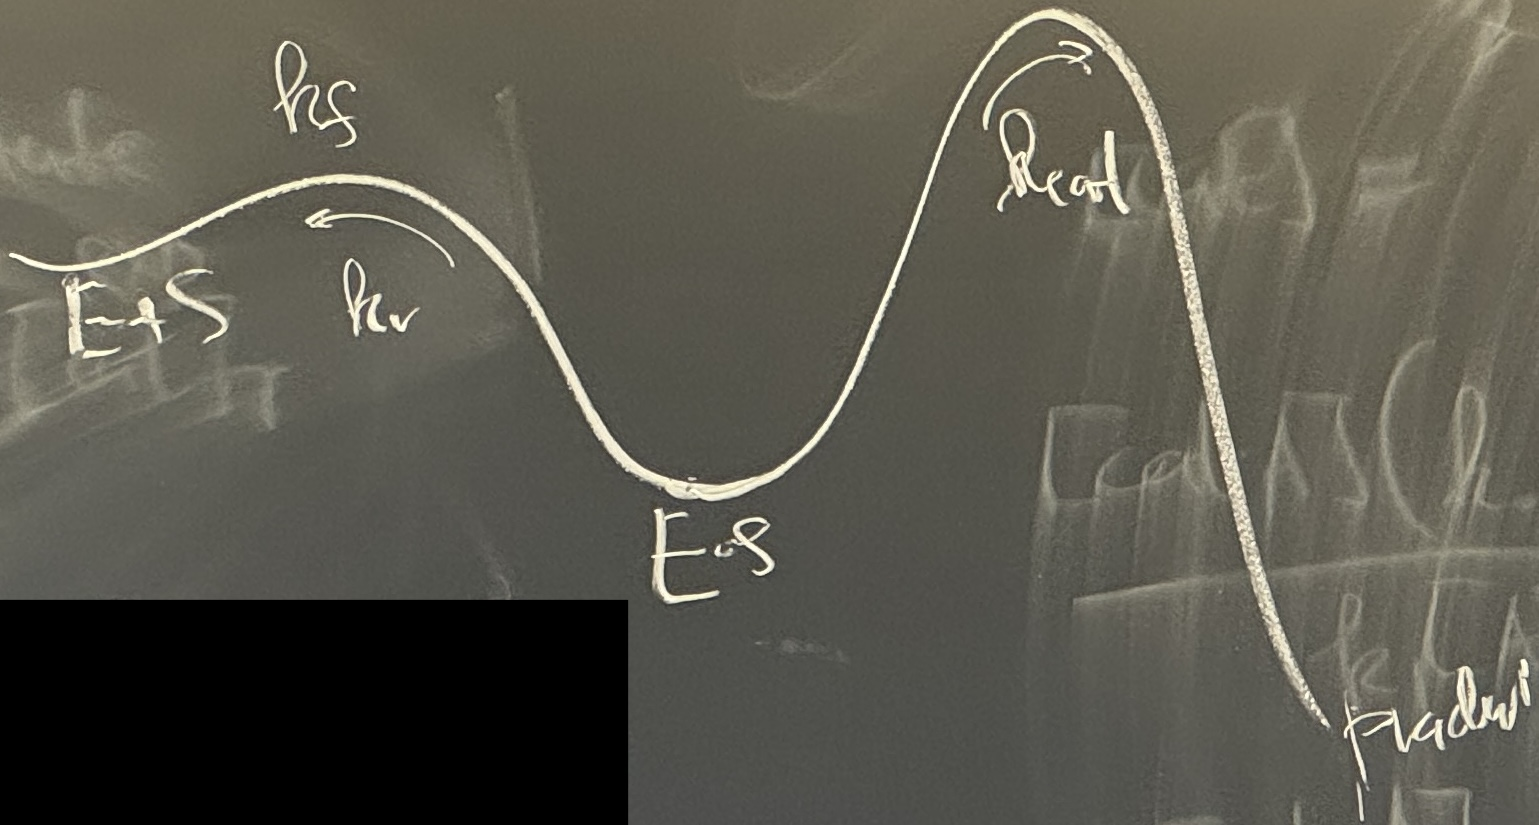
\includegraphics[width=0.95\linewidth]{MMkinb.JPG}
            \caption{First-order.}
            \label{fig:MMkinb}
        \end{subfigure}
        \caption{Michaelis-Menten kinetic regimes.}
        \label{fig:MMkin}
    \end{figure}
    \begin{itemize}
        \item Enzymes can be characterized according the Michaelis constant $K_m$ and the intrinsic rate constant $k_\text{cat}$.
        \item When we're zeroeth order in the substrate, we have one kinetic regime.
        \item When we're first-order in the substrate, we have a kinetic regime that's more like quasi-equilibrium!
        \item How well the enzyme binds the substrate is a measure of how efficient the catalyst is.
    \end{itemize}
    \item When $k_r\gg k_\text{cat}$,
    \begin{equation*}
        K_m \approx \frac{k_r}{k_f} = K_D
    \end{equation*}
    \begin{itemize}
        \item This ratio measures how well the enzyme binds to the substrate.
    \end{itemize}
    \item When $k_\text{cat}\gg k_r$,
    \begin{equation*}
        K_m \approx \frac{k_\text{cat}}{K_m} =: \text{specificity constant}
    \end{equation*}
    \begin{itemize}
        \item These ratios can be analyzed as the specificity constant for a specific enzyme.
        \item Describes an enzyme's preference (both in terms of binding and reactivity) for one substrate over another.
    \end{itemize}
    \item Example: Fumerase (responsible for redox transport).
    \begin{itemize}
        \item $K_m=\num{5e-6}$, and $k_\text{cat}=\num{8e2}$, so SC is $\num{e7}$.
    \end{itemize}
    \item Example: Carbonic anhydrase.
    \begin{itemize}
        \item $K_m=\num{2.6e-2}$, and $k_\text{cat}=\num{4e5}$, so SC is $\num{e8}$.
    \end{itemize}
    \item So for great catalysis, you want the catalyst to find substrate quickly and immediately turn it over.
    \begin{itemize}
        \item These two catalysts operate near the diffusion limit (which is ideal); they are near-perfect.
    \end{itemize}
    \item References.
    \begin{itemize}
        \item \textcite{bib:EnzymeCat}.
        \item A beautiful piece of literature; the touchstone for biological catalysis, per Alex.
    \end{itemize}
\end{itemize}




\end{document}